\section{Calculating complexity in relational algebra}
A method for calculating complexity of relational algebra trees was suggested
by \O ystein Torbj\o rnsen at FAST. This method is based on the assumption
that the algebra will be executed on an implementation written in Java or a
similar object oriented language. Not withstanding the benefits of compile-level
optimisations and other ways to increase performance such as caching, this
method of calculation defines complexity as creation of new objects in run-time. 

This definition of complexity does \textit{not} account
for disk I/O, nor is it a direct measurement of performance. However, given
an algebra tree which is to be executed on some known host implementation, it
may give an indication of spending of time and computational resources.

\subsection{Definitions}
\begin{myDefinition}
A \textbf{post} is an in-memory object which contains a value and a mapping to
an attribute name in a relation
\label{definition:relalg_post}
\end{myDefinition}

\begin{myDefinition}
A \textbf{tuple} is defined as an in-memory object which contains a set of
\textit{posts} (definition \ref{definition:relalg_post}), where each post
contains a value for some given attribute in the relation
\label{definition:relalg_tuple}
\end{myDefinition}

\begin{myDefinition}
Measurement of \textbf{complexity} is defined as that for some given operator
$\alpha$, counting the following operations performed by the operator:
\begin{itemize}
  \item Creation of new \textbf{tuples} (definition
  \ref{definition:relalg_tuple})
  \item Creation of new \textbf{posts} (definition \ref{definition:relalg_post})
\end{itemize}
The integer sum of counting these operations (from and including 1 and up)
defines the \textbf{complexity} for that given operator. Further, the sum of
all the complexity sums in some given relational algebra tree defines the
\textbf{complexity sum} for that given tree.
\label{definition:relalg_complexity}
\end{myDefinition}

%\usepackage{graphics} is needed for \includegraphics
\begin{figure}[htp]
\begin{center}
  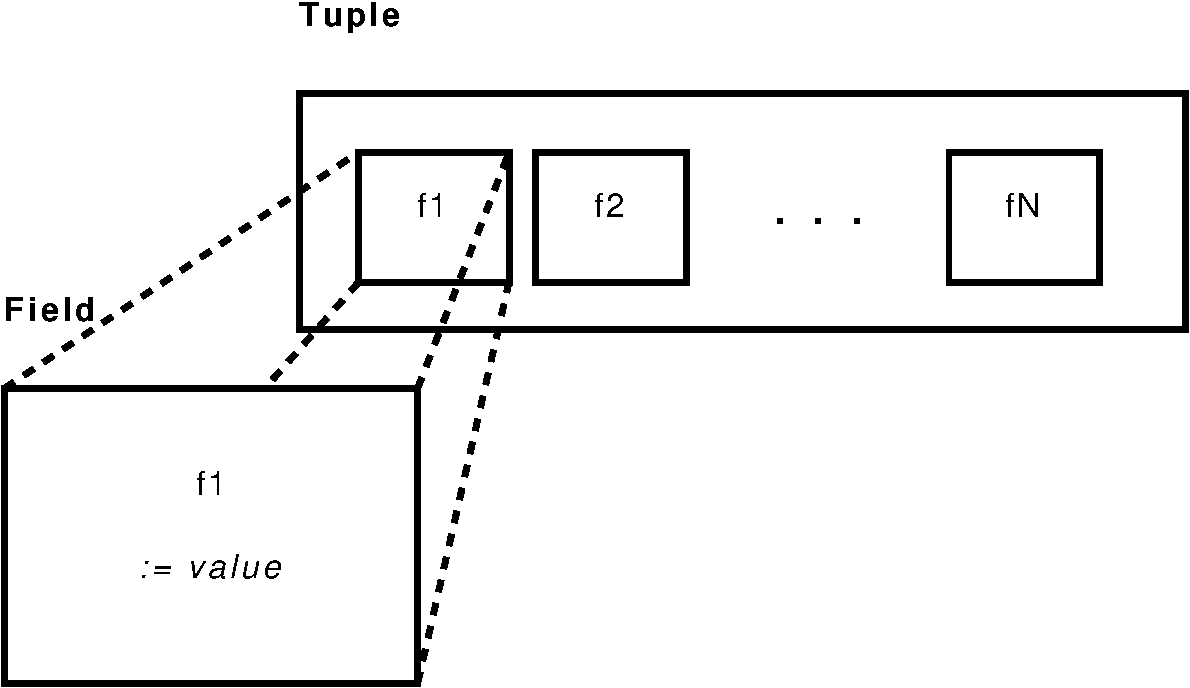
\includegraphics[width=0.7\textwidth]{diagrams/tuple_post}
  \caption[Tuple/Post]{The structure of a \textit{tuple} with \textit{posts}}
  \label{fig:method:tuple_post}
\end{center}
\end{figure}